\documentclass{article}
\usepackage{graphicx}
\usepackage{xcolor}
\usepackage{standalone}
\usepackage{tikz}
\usetikzlibrary{arrows.meta, positioning, shapes.geometric, calc, fit, backgrounds}
\usepackage{amsmath, amssymb}
\usepackage{hyperref}
\hypersetup{colorlinks=true, urlcolor=blue, linkcolor=black, citecolor=black}

%% ============================================================
%% Probability parameters for the cost-chain flowchart
%% These feed figures/cost_chain_flowchart.tex, which is \input below
%% ============================================================
% Colorimetric (roadside) test
\newcommand{\pColorFP}{0.037}     % colorimetric false-positive rate
\newcommand{\pColorTN}{0.963}     % 1 - pColorFP (true neg. / false neg.)
% Handheld (station) confirmatory test -- only used "w/ law"
\newcommand{\pHandheldFP}{0.001}  % handheld FP rate (passes through to booking)
% Main chain transitions
\newcommand{\pBookFromArr}{1.00}  % Arrest -> Booking (w/o law scenario)
\newcommand{\pArrFromBook}{1.00}  % Booking -> Arraignment
\newcommand{\pPreFromArr}{1.00}   % Arraignment -> Pretrial
\newcommand{\pBrFromPre}{0.95}    % Pretrial -> Bail Review
\newcommand{\pPassBr}{0.95}       % Bail Review -> bond fork (1 - dismissed)
\newcommand{\pDisBr}{0.05}        % Dismissed at bail review
\newcommand{\pRel}{0.90}          % Released on recog.
\newcommand{\pHome}{0.05}         % Home confinement
\newcommand{\pHeld}{0.05}         % Held in custody
\newcommand{\pPrep}{1.00}         % Bond fork -> Case Prep
\newcommand{\pPres}{0.34}         % Case Prep -> Case Presentation
\newcommand{\pDisCp}{0.66}        % Charges dismissed at case prep
\newcommand{\pCoFromPres}{0.38}   % Case Presentation -> Costed Outcome
\newcommand{\pNoCost}{0.62}       % No-cost outcome
% Cumulative reach (per arrest, baseline / "w/o law" scenario)
\newcommand{\PArrest}{1.000}
\newcommand{\PBook}{1.000}
\newcommand{\PArr}{1.000}
\newcommand{\PPre}{0.950}
\newcommand{\PBr}{0.950}
\newcommand{\PCp}{0.903}
\newcommand{\PCpres}{0.307}
\newcommand{\PCo}{0.117}

%% ============================================================
%% Auto-generated headline numbers (written by make_exhibits.do).
%% \providecommand fallbacks let the document compile before the
%% Stata pipeline has been run; real values overwrite them on \input.
%% ============================================================
\IfFileExists{figures/results_macros.tex}{% Auto-generated by make_exhibits.do -- do not edit by hand.
\newcommand{\resNyears}{6}
\newcommand{\resMinYear}{2019}
\newcommand{\resMaxYear}{2024}
\newcommand{\resArrestsTotal}{204,156}
\newcommand{\resArrestsAnnual}{34,026}
\newcommand{\resPolicyCost}{997,215}
\newcommand{\resBenefitBase}{1,455,795}
\newcommand{\resBenefitMid}{3,513,035}
\newcommand{\resNetBase}{458,580}
\newcommand{\resNetMid}{2,515,820}
\newcommand{\resBcrBase}{1.5}
\newcommand{\resBcrMid}{3.5}
\newcommand{\resCostMar}{1,551}
\newcommand{\resCostCoc}{3,440}
\newcommand{\resCostSyn}{1,663}
\newcommand{\resCostOth}{2,603}
\newcommand{\resCostMarFP}{57}
\newcommand{\resPctTests}{49.9}
}{}
\providecommand{\resNyears}{6}
\providecommand{\resMinYear}{2019}
\providecommand{\resMaxYear}{2024}
\providecommand{\resArrestsTotal}{--}
\providecommand{\resArrestsAnnual}{--}
\providecommand{\resPolicyCost}{797,772}
\providecommand{\resBenefitBase}{--}
\providecommand{\resBenefitMid}{--}
\providecommand{\resNetBase}{--}
\providecommand{\resNetMid}{--}
\providecommand{\resBcrBase}{--}
\providecommand{\resBcrMid}{--}
\providecommand{\resCostMar}{--}
\providecommand{\resCostCoc}{--}
\providecommand{\resCostSyn}{--}
\providecommand{\resCostOth}{--}
\providecommand{\resCostMarFP}{57}
\providecommand{\resPctTests}{49.9}

\title{The Cost and Benefit of NC HB 868:\\ Methodology and Results}
\author{Spencer Cooper-Ohm, Jeff DeSimone\\ \\Duke University Economics Analytics Laboratory}
\date{\today}

\begin{document}

\maketitle

\section{Overview}
Roadside colorimetric drug tests are cheap, ubiquitous, and unreliable. The Quattrone Center's review of field drug testing, \href{https://scholarship.law.upenn.edu/qc_reports/26/}{\emph{Guilty Until Proven Innocent}}, documents that these \$2 chemical reagent kits have false positive rates that routinely furnish the probable cause for arrest, booking, and even guilty pleas. Drawing on surveyed agencies, the Quattrone Center estimates that roughly 49.9\% of drug arrests rest on a colorimetric test, and that approximately 3.7\% of police-department colorimetric tests that indicate drug use are false positives. In addition to the social costs of arresting the innocent for drug-related crimes they did not commit, there is a large economic cost associated with erroneously pursuing an arrest and prosecution based on the results of a false positive colorimetric test.

In this document, we evaluate the economic consequences of the policy proposed by NC HB868, which prevents the use of presumptive colorimetric drug tests to find a probable cause for an arrest. Using historical arrest data from North Carolina and estimates of judicial costs from a nearby state, we show the average wasted cost to the state from using colorimetric tests is nearly \$1.5 million under the most conservative estimate, and upwards of \$3.5 million under average judicial costs and progression through the criminal justice system. Additionally, we calculate the cost of one possible (but by no means the only) equivalent drug testing scheme that would eliminate the need for colorimetric tests, and would save the state roughly \$500,000 annually by our most conservative estimates.

In Section 2, we detail our methodology calculating the annual government waste associated with colorimetric testing. In Section 3, we examine the financial implications of adopting a policy of using handheld Raman spectrometers (such as the \href{https://www.thermofisher.com/us/en/home/industrial/safety-security-threat-detection/instruments/trunarc-handheld-narcotics-analyzer.html}{TruNarc analyzer}) at all booking locations in North Carolina. Throughout, we adopt assumptions that are deliberately conservative, so that the estimated benefit is a lower bound. We count only direct governmental monetary costs that are avoided; no social or private benefits to innocent suspects who are spared erroneous arrest are included.

\section{Assessing Waste Associated with Colorimetric Tests}
\subsection{Summary}
To estimate the judicial cost incurred by a drug-related arrest, prosecution, and potential conviction, we use two sources:
\begin{itemize}
    \item \href{https://americanhealth.jhu.edu/sites/default/files/estimating-economic-costs-prosecuting-simple-drug-possession-baltimore-city-april-2023.pdf}{2023 estimates of drug prosecution costs in Baltimore}. This report contains cost estimates of each step of the criminal process from arrest to conviction, and provides probabilities for a given defendant reaching the next step of the process conditional on reaching the step before it. We use the Baltimore report because it provides a complete picture of costs associated with the prosecution process and provides probabilities for moving between steps, all in a city relatively proximate to North Carolina. No such report exists for North Carolina that we are aware of.\footnote{If this data becomes avaliable, or if the reader wishes to test alternate parameters for any step of this analysis, the params.do file in the associated Github contains all the cost and probability parameters we use for our analysis. The values can easily be changed and the Stata script re-ran.} For our baseline specification we take the lower-bound estimate for all values in this report---the lowest probability that a defendant advances through each step, and the lowest estimated cost at each step. This ensures that our baseline estimate of the cost-saving properties of the policy is as conservative as possible.
    \item North Carolina \href{https://www.openicpsr.org/openicpsr/project/118281/version/V11/view}{NIBRS} data from \resMinYear{} to \resMaxYear{}. We analyze all arrest records that include seized drugs within the NIBRS property segment. We use North Carolina sentencing statistics from 2024 to construct a weighted average cost of each drug-related disposition, assuming when possible that judges administer the lowest possible sentence within the empirically observed range.
\end{itemize}

\subsection{Cost Construction}
Our estimates are reproducible by downloading publicly available NIBRS data and using the Stata code in this document's associated Github. We briefly describe the sample construction below:

\begin{enumerate}
    \item \textbf{Build the arrest panel.} 
    For arrest data, we use the North Carolina NIBRS from \resMinYear{}--\resMaxYear{}. During this period, roughly 98\% of North Carolinians were covered by NIBRS-reporting agencies. We restrict the data to incidents involving the seizure of drugs or narcotics, and remove incidents not involving a specific named drug from the sample (all false-positive colorimetric tests will result in the identification of at least one drug). We also make the conservative decision to restrict the sample to arrests in which drugs or narcotics are seized.\footnote{i.e. we exclude arrests in the scenario that a colorimetric test is used on suspected drugs, the test comes up positive, and the officer does not seize the drugs.}
\item \textbf{Classify drug charges.} Each NIBRS incident details the type and quantity of each drug seized in an arrest. We determine the offense level associated with each drug using \href{https://www.ncleg.net/EnactedLegislation/Statutes/HTML/BySection/Chapter_90/GS_90-95.html}{NC G.S.\ 90-95}. For example, an incident involving 0.4 ounces of marijuana and 1 pound of cocaine would be classified as a Class 3 misdemeanor for the marijuana under G.S.\ 90-95(d)(4) and as a Class D trafficking felony for the cocaine under G.S.\ 90-95(h)(3). For each incident, we assume that the highest offense is charged and all other charges are dropped.\footnote{Again, this makes the conservative assumption, rather than the very real possibility that an arrestee accumulates multiple charges for a single instance of arrest} Thus, the above example would be coded as a Class D felony. This offense classification becomes important when we calculate the cost associated with disposition in step 4 of the sample construction.



    \item \textbf{Judicial costs.}
        We assemble the expected cost of each arrest as the probability-weighted sum of every stage of the criminal process (Figure~\ref{fig:flowchart}), and from it the expected \emph{waste}---the share of that cost attributable to colorimetric false positives.
    For analysis purposes, we ignore the cost of any true-positive colorimetric test that results in an arrest (the money the state spends on these arrests is a justified cause) or any false-negative tests (cost of colorimetric tests and time to test is minimal). We focus on false-positive colorimetric test-based arrests, the resulting costs of which are effectively money lost on arresting, prosecuting, and imprisoning an innocent person.

When a colorimetric test results in a false positive, it triggers a pipeline of procedures, with each step in the pipeline incurring a cost. Those implicated by colorimetric tests are arrested, booked, arraigned, and put through the bail process. Then, the state must spend additional funds on case preparation and presentation (including plea procedures). If the defendant is found guilty, money must be spent on dispositions. We estimate the expected cost of an arrest as the sum of the cost of each step $i$ times the cumulative probability $P$ of reaching $i$. The probabilities and costs used in our baseline model are shown in Figure~\ref{fig:flowchart}.

\begin{figure}[p]
  \centering
  \resizebox{0.8\textwidth}{!}{% cost_chain_flowchart.tex
% Standalone TikZ flowchart of the per-arrest cost chain modeled in
% estimate_costs.do. Compile with: pdflatex cost_chain_flowchart.tex
%
% Each stage box: stage name + per-incidence cost (incurred if reached).
% Each forward edge: transition probability to the next stage.
% Dashed edges: exits (dismissal / no-cost outcome / exoneration).
% Sentence cost is shown generalized -- per-class values come from the SPAC
% empirical lookup and trafficking statute (see sentence_lengths.do).

\documentclass[border=10pt]{standalone}
\usepackage{tikz}
\usepackage{amsmath, amssymb}
\usetikzlibrary{arrows.meta, positioning, shapes.geometric, calc, fit, backgrounds}

%% ============================================================
%% Probability parameters -- edit values here to update diagram.
%% These live in the preamble so this file compiles on its own
%% (pdflatex cost_chain_flowchart.tex). When this file is \input
%% into main.tex / methodology.tex via the standalone package,
%% this preamble is ignored and the host document's own copies of
%% these macros are used instead -- so there is no clash.
%% ============================================================
% Colorimetric (roadside) test
\newcommand{\pColorFP}{0.037}     % colorimetric false-positive rate
\newcommand{\pColorTN}{0.963}     % 1 - pColorFP (true neg. / false neg.)
% Handheld (station) confirmatory test -- only used "w/ law"
\newcommand{\pHandheldFP}{0.001}  % handheld FP rate (passes through to booking)
% Main chain transitions
\newcommand{\pBookFromArr}{1.00}  % Arrest -> Booking (w/o law scenario)
\newcommand{\pArrFromBook}{1.00}  % Booking -> Arraignment
\newcommand{\pPreFromArr}{1.00}   % Arraignment -> Pretrial
\newcommand{\pBrFromPre}{0.95}    % Pretrial -> Bail Review
\newcommand{\pPassBr}{0.95}       % Bail Review -> bond fork (1 - dismissed)
\newcommand{\pDisBr}{0.05}        % Dismissed at bail review
\newcommand{\pRel}{0.90}          % Released on recog.
\newcommand{\pHome}{0.05}         % Home confinement
\newcommand{\pHeld}{0.05}         % Held in custody
\newcommand{\pPrep}{1.00}         % Bond fork -> Case Prep
\newcommand{\pPres}{0.34}         % Case Prep -> Case Presentation
\newcommand{\pDisCp}{0.66}        % Charges dismissed at case prep
\newcommand{\pCoFromPres}{0.38}   % Case Presentation -> Costed Outcome
\newcommand{\pNoCost}{0.62}       % No-cost outcome
% Cumulative reach (per arrest, baseline / "w/o law" scenario)
\newcommand{\PArrest}{1.000}
\newcommand{\PBook}{1.000}
\newcommand{\PArr}{1.000}
\newcommand{\PPre}{0.950}
\newcommand{\PBr}{0.950}
\newcommand{\PCp}{0.903}
\newcommand{\PCpres}{0.307}
\newcommand{\PCo}{0.117}

\begin{document}

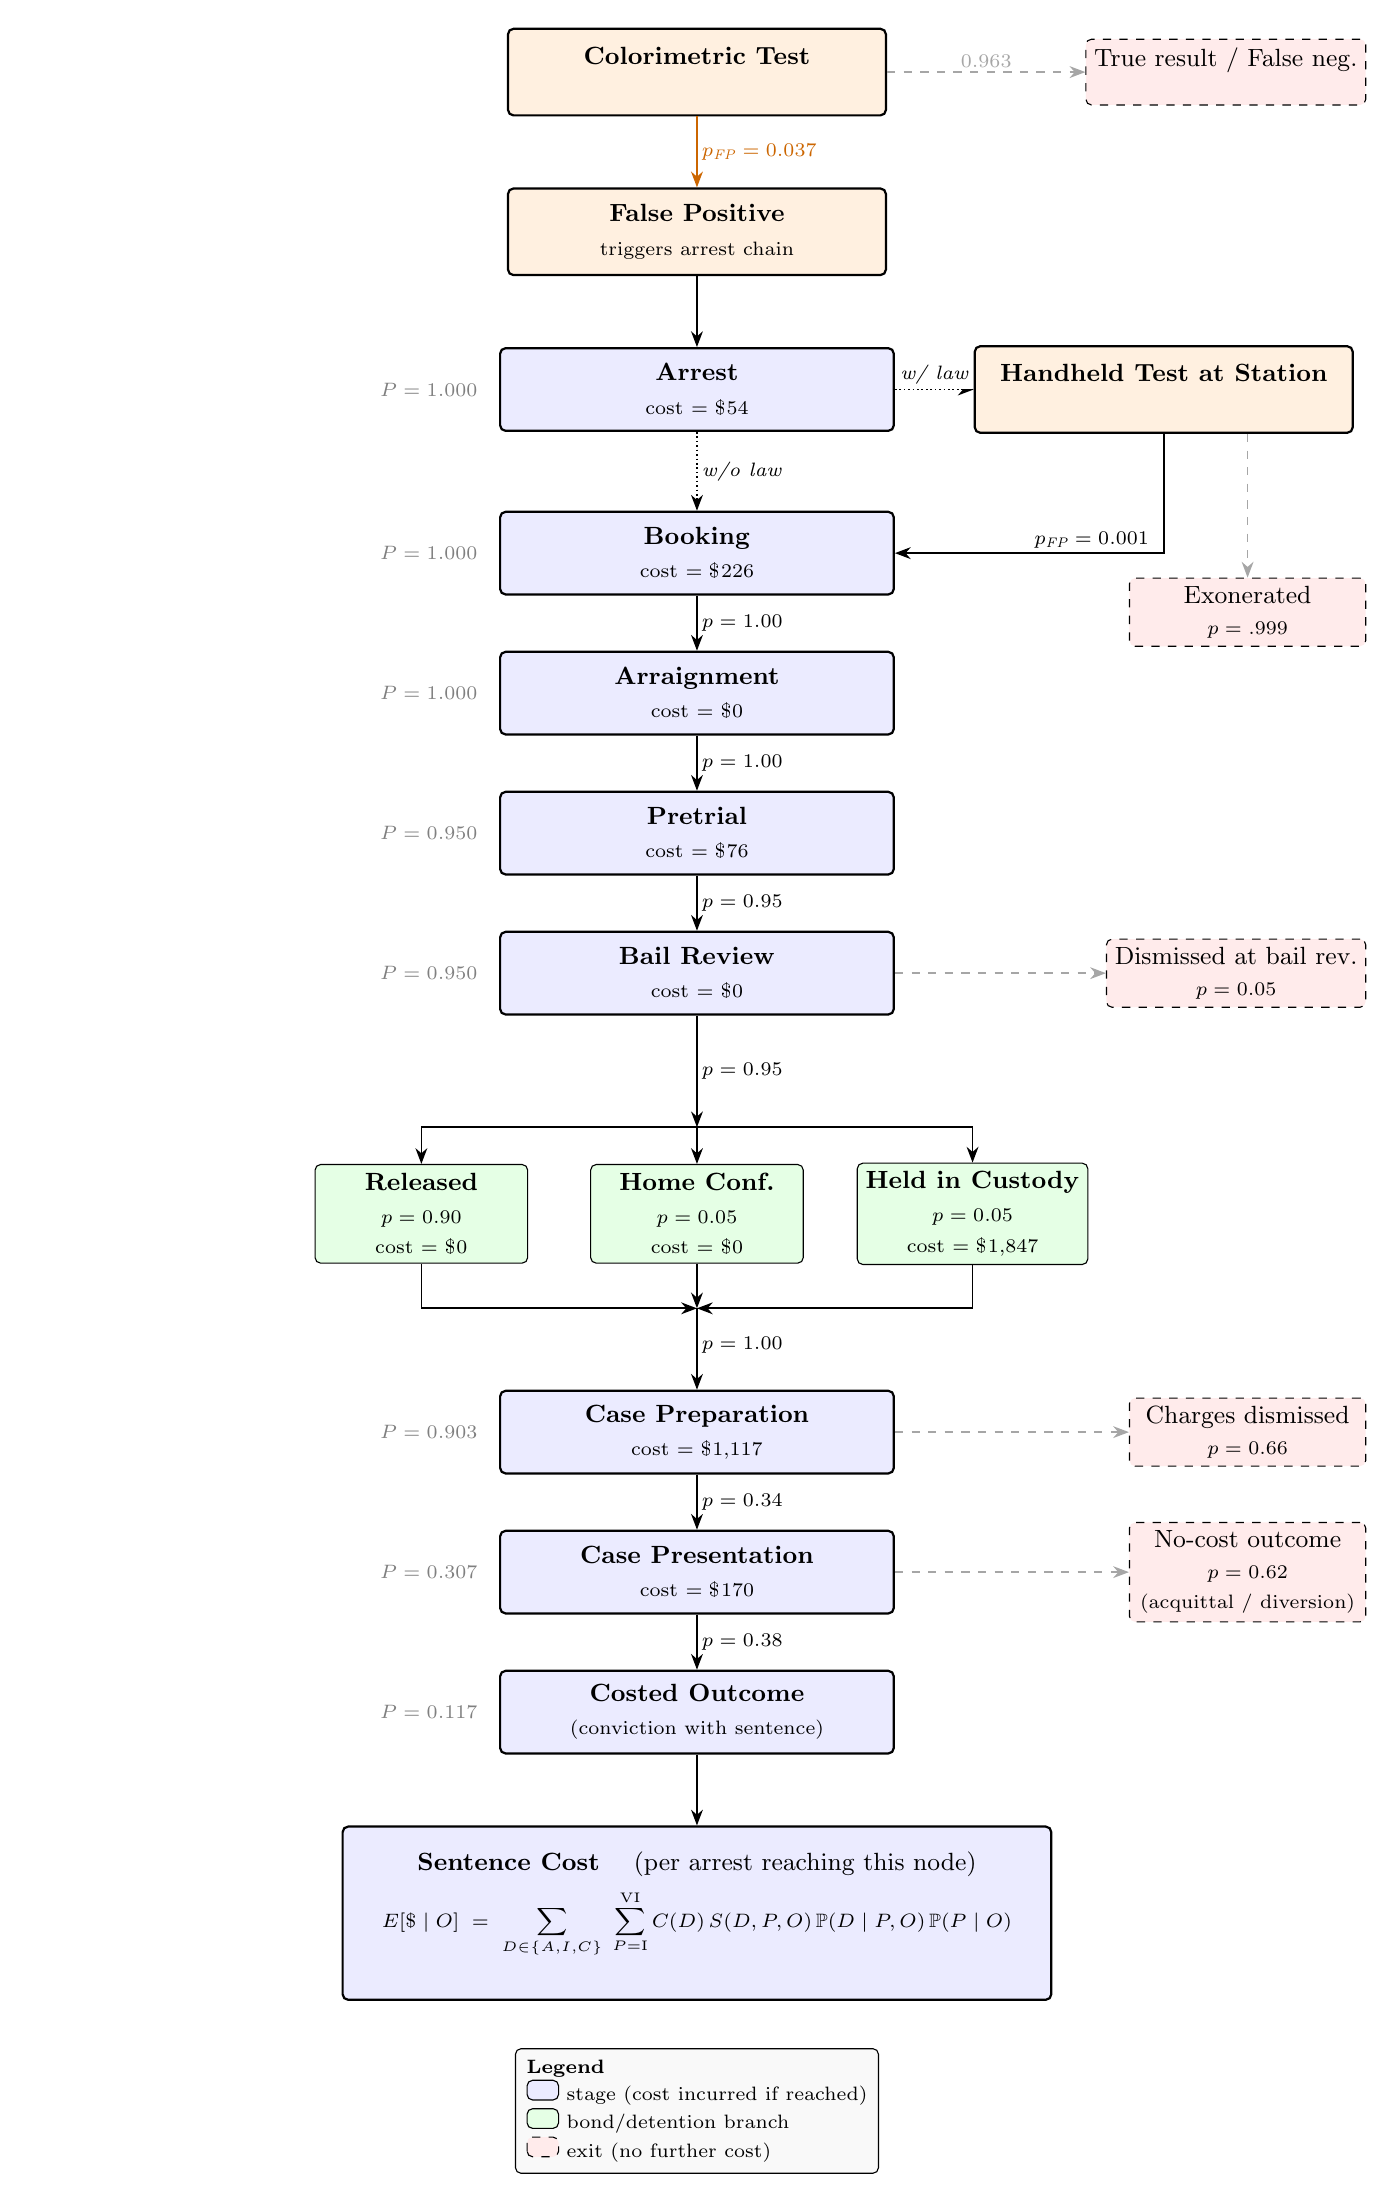
\begin{tikzpicture}[
  every node/.style = {font=\small, align=center},
  stage/.style    = {rectangle, draw, rounded corners=2pt, fill=blue!8,
                     thick, minimum width=5cm, minimum height=1.05cm,
                     inner sep=4pt},
  bond/.style     = {rectangle, draw, rounded corners=2pt, fill=green!10,
                     minimum width=2.7cm, minimum height=1.1cm, inner sep=3pt},
  exit/.style     = {rectangle, draw, rounded corners=2pt, fill=red!8,
                     dashed, minimum width=3cm, minimum height=0.8cm,
                     inner sep=3pt},
  sentence/.style = {rectangle, draw, rounded corners=2pt, fill=blue!8,
                     thick, minimum width=9cm, minimum height=2.2cm,
                     inner sep=6pt},
  colortest/.style= {rectangle, draw, rounded corners=2pt, fill=orange!12,
                     thick, minimum width=4.8cm, minimum height=1.1cm,
                     inner sep=4pt},
  arr/.style      = {-Stealth, semithick},
  dotarr/.style   = {-Stealth, semithick, densely dotted},
  exitarr/.style  = {-Stealth, semithick, dashed, gray!70},
  elab/.style     = {font=\scriptsize\itshape, fill=white, inner sep=1.5pt}
]

%% -------- Pre-arrest colormetric stack (above Arrest) --------
\node[colortest]                       (cm) at (0, 4.2) {\textbf{Colorimetric Test}\\[1pt]
                                                          };
\node[colortest,
      below=0.9cm of cm]               (fp) {\textbf{False Positive}\\[1pt]
                                              \scriptsize triggers arrest chain};

%% -------- Main vertical chain --------
\node[stage, below=0.9cm of fp]  (a)  {\textbf{Arrest}\\[1pt]
                                        \scriptsize cost = \$54};
\node[stage, below=1.0cm of a]   (b)  {\textbf{Booking}\\[1pt]
                                        \scriptsize cost = \$226};
\node[stage, below=0.7cm of b]   (ar) {\textbf{Arraignment}\\[1pt]
                                        \scriptsize cost = \$0};
\node[stage, below=0.7cm of ar]  (pt) {\textbf{Pretrial}\\[1pt]
                                        \scriptsize cost = \$76};
\node[stage, below=0.7cm of pt]  (br) {\textbf{Bail Review}\\[1pt]
                                        \scriptsize cost = \$0};

%% -------- Handheld station test (right of Arrest) --------
\node[colortest, right=1.0cm of a]   (hh) {\textbf{Handheld Test at Station}\\[1pt]
                                            };
%% Shared right-edge coordinate -- every exit box is anchored east at this x,
%% so their right edges all line up regardless of internal width.
\coordinate (exitR) at (8.5, 0);
\node[exit, anchor=east] (tn)     at (exitR |- cm)    {True result / False neg.\\};
\node[exit, anchor=east] (exon)   at ($(exitR |- b) - (0,0.75)$)     {Exonerated\\ \scriptsize $p = .999$};

%% -------- Bond fork (3 parallel branches) --------
\node[bond] (rel)  at (-3.5, -10.3) {\textbf{Released}\\[1pt]
                                     \scriptsize $p=\pRel$\\ \scriptsize cost = \$0};
\node[bond] (home) at ( 0,   -10.3) {\textbf{Home Conf.}\\[1pt]
                                     \scriptsize $p=\pHome$\\ \scriptsize cost = \$0};
\node[bond] (held) at ( 3.5, -10.3) {\textbf{Held in Custody}\\[1pt]
                                     \scriptsize $p=\pHeld$\\ \scriptsize cost = \$1{,}847};

%% -------- Resume main column --------
\node[stage, below=1.6cm of home]  (cp)   {\textbf{Case Preparation}\\[1pt]
                                            \scriptsize cost = \$1{,}117};
\node[stage, below=0.7cm of cp]    (cpres){\textbf{Case Presentation}\\[1pt]
                                            \scriptsize cost = \$170};
\node[stage, below=0.7cm of cpres] (co)   {\textbf{Costed Outcome}\\[1pt]
                                            \scriptsize (conviction with sentence)};

%% -------- Generalized sentence cost --------
\node[sentence, below=0.9cm of co] (sent) {%
  \textbf{Sentence Cost} \quad (per arrest reaching this node) \\[4pt]
  \scriptsize $\displaystyle
    E[\$\mid O] \;=\;
        \sum_{D \in \{A,I,C\}} \;\sum_{P = \text{I}}^{\text{VI}}
        C(D)\,S(D, P, O)\,\mathbb{P}(D \mid P, O)\,\mathbb{P}(P \mid O)$ \\[5pt]
};

%% -------- Right-side exits (aligned vertically to their source stage) --------
\node[exit, anchor=east] (dis_br)  at (exitR |- br)    {Dismissed at bail rev.\\ \scriptsize $p=\pDisBr$};
\node[exit, anchor=east] (dis_cp)  at (exitR |- cp)    {Charges dismissed\\ \scriptsize $p=\pDisCp$};
\node[exit, anchor=east] (no_cost) at (exitR |- cpres) {No-cost outcome\\ \scriptsize $p=\pNoCost$\\ \scriptsize (acquittal / diversion)};

%% -------- Colormetric -> FP / TN edges --------
\draw[arr, orange!80!black] (cm) -- node[elab, right]{$p_{\text{FP}}=\pColorFP$} (fp);
\draw[exitarr] (cm) -- node[elab, above]{$\pColorTN$} (tn);
\draw[arr] (fp) -- (a);

%% -------- Arrest -> Booking fork (w/o law direct, w/ law via handheld) --------
\draw[dotarr] (a) -- node[elab, right]{w/o law} (b);
\draw[dotarr] (a) -- node[elab, above]{w/ law} (hh);
\draw[arr] (hh.south) |- node[elab, above right, pos=0.75]{$p_{\text{FP}}=\pHandheldFP$} (b.east);
\draw[exitarr] (hh.south -| exon) -- (exon);

%% -------- Forward arrows with prob labels --------
\draw[arr] (b)  -- node[elab, right]{$p=\pArrFromBook$} (ar);
\draw[arr] (ar) -- node[elab, right]{$p=\pPreFromArr$} (pt);
\draw[arr] (pt) -- node[elab, right]{$p=\pBrFromPre$} (br);

%% Bail review --> bond fork (with pPassBr = 1 - dismissed)
\coordinate (fork) at (0, -9.2);
\draw[arr] (br.south) -- node[elab, right]{$p=\pPassBr$} (fork);
\draw[arr] (fork) -| (rel.north);
\draw[arr] (fork) -- (home.north);
\draw[arr] (fork) -| (held.north);

%% Bond branches converge into Case Prep
\coordinate (merge) at (0, -11.5);
\draw[arr] (rel.south)  |- (merge);
\draw[arr] (home.south) -- (merge);
\draw[arr] (held.south) |- (merge);
\draw[arr] (merge) -- node[elab, right, pos=0.45]{$p=\pPrep$} (cp);

\draw[arr] (cp)    -- node[elab, right]{$p=\pPres$} (cpres);
\draw[arr] (cpres) -- node[elab, right]{$p=\pCoFromPres$} (co);
\draw[arr] (co)    -- (sent);

%% Dashed exits
\draw[exitarr] (br)    -- (dis_br);
\draw[exitarr] (cp)    -- (dis_cp);
\draw[exitarr] (cpres) -- (no_cost);

%% -------- Cumulative reach-probability annotations (left column) --------
\node[left=0.15cm of a,     font=\scriptsize\color{gray}] {$P=\PArrest$};
\node[left=0.15cm of b,     font=\scriptsize\color{gray}] {$P=\PBook$};
\node[left=0.15cm of ar,    font=\scriptsize\color{gray}] {$P=\PArr$};
\node[left=0.15cm of pt,    font=\scriptsize\color{gray}] {$P=\PPre$};
\node[left=0.15cm of br,    font=\scriptsize\color{gray}] {$P=\PBr$};
\node[left=0.15cm of cp,    font=\scriptsize\color{gray}] {$P=\PCp$};
\node[left=0.15cm of cpres, font=\scriptsize\color{gray}] {$P=\PCpres$};
\node[left=0.15cm of co,    font=\scriptsize\color{gray}] {$P=\PCo$};

%% -------- Legend --------
\node[draw, rounded corners=2pt, fill=gray!5, inner sep=4pt,
      below=0.6cm of sent.south,
      anchor=north, font=\scriptsize, align=left] (leg) {%
   \textbf{Legend} \\
   \tikz\draw[fill=blue!8]   (0,0) rectangle (0.4,0.25);\ stage (cost incurred if reached) \\
   \tikz\draw[fill=green!10] (0,0) rectangle (0.4,0.25);\ bond/detention branch \\
   \tikz\draw[fill=red!8, dashed] (0,0) rectangle (0.4,0.25);\ exit (no further cost)};

%% Symmetric left padding so the bounding box (and hence the figure) is
%% centered on the main vertical chain at x=0, mirroring the right-side
%% exits/handheld extent. Invisible -- only affects the bounding box.
\path (-8.5, 0);

\end{tikzpicture}

\end{document}
}
  \caption{Per-Arrest Cost Chain.}
  \label{fig:flowchart}
\end{figure}

    \item \textbf{Disposition costs.} To determine disposition type and length resulting from a guilty outcome, we rely on Tables 4 and 19 from the \href{https://www.nccourts.gov/assets/documents/publications/SPAC-FY-2024-Statistical-Report.pdf}{SPAC FY-2024 Statistical Report}, which provide the prior record level of North Carolina defendants convicted at each offense class, as well as the disposition type and sentence range of each offense class conditional on prior record. Table~\ref{tab:spac_class_d} reproduces the Class~D row of SPAC Table~4 (the relevant row for the cocaine example above).

\begin{table}[h]
\centering
\small
\caption{An example row (Class D Felony) from the SPAC Report Table 4: convictions by prior record level and disposition type.}
\label{tab:spac_class_d}
\resizebox{\textwidth}{!}{%
\begin{tabular}{c|cccccc|c}
\hline
 & \multicolumn{6}{c|}{Prior Record Level} & \\
 & I & II & III & IV & V & VI & Total \\
 & 0--1 pt & 2--5 pt & 6--9 pt & 10--13 pt & 14--17 pt & 18+ pt & \\
\hline
Community     & 0          & 0           & 0           & 0           & 0          & 0           & 0 \\
Intermediate  & 19 (6\%)   & 0           & 0           & 0           & 0          & 0           & 19 (2\%) \\
Active        & 308 (94\%) & 139 (100\%) & 107 (100\%) & 102 (100\%) & 73 (100\%) & 106 (100\%) & 835 (98\%) \\
\hline
Total $n$     & 327        & 139         & 107         & 102         & 73         & 106         & 854 \\
Avg min (mo)  & 52         & 59          & 66          & 75          & 83         & 98          & -- \\
Avg max (mo)  & 77         & 84          & 92          & 103         & 114        & 131         & -- \\
\hline
\end{tabular}%
}
\end{table}

The expected sentence cost for an offense at class~$O$ is
$$
    E[\$\mid O] \;=\;
        \sum_{D \in \{A,I,C\}}\; \sum_{P = \text{I}}^{\text{VI}}
        C(D)\,S(D, P, O)\,\mathbb{P}(D\mid P, O)\,\mathbb{P}(P\mid O),
$$
where:
\begin{itemize}
    \item $D \in \{A, I, C\}$ is the disposition type: active (prison), intermediate, or community punishment. $C(D)$ is the monthly cost associated with each disposition.
    \item $P \in \{\text{I}, \dots, \text{VI}\}$ is the prior record level and $O$ is the offense class.
    \item $S(D, P, O)$ is the expected sentence length in months. For active sentences this is the SPAC Table~4 average-minimum-sentence cell. For intermediate and community probation, the length is the minimum of the default range in \href{https://www.ncleg.net/EnactedLegislation/Statutes/HTML/BySection/Chapter_15A/GS_15A-1343.2.html}{G.S.\ 15A-1343.2(d)}.
\end{itemize}
Trafficking offenses are the exception: G.S.\ 90-95(h) mandates fixed minimums regardless of prior record or judicial discretion, so for those rows we override the empirical mix with a 100\% active disposition at the statutory sentence.

\end{enumerate}


\section{The Cost of Colormetrics}\label{sec:results}
We repeatedly run our cost estimate under several assumption sets. Because the Baltimore report provides ranges rather than point estimates, we report results under five specifications. Each varies one family of assumptions while holding the others at their conservative floor, except the last, which moves all values to their midpoints:
\begin{itemize}
    \item \textbf{Baseline}: lowest stage-transition probabilities, lowest stage costs, and shortest (minimum) sentences. This is the most conservative case.
    \item \textbf{High Probabilities}: highest probabilities of advancing through the system; costs and sentences at their floor.
    \item \textbf{High Cost}: highest per-stage costs; probabilities and sentences at their floor.
    \item \textbf{High Sentencing}: longest (maximum) sentences; probabilities and costs at their floor.
    \item \textbf{All Midpoints}: probabilities, costs, and sentence lengths all set to the midpoint of their ranges.
\end{itemize}

Table~\ref{tab:cost_by_type} reports the resulting expected legal-system cost per arrest, broken out by the four major drug categories (marijuana; opium or cocaine; synthetic narcotics; and other dangerous non-narcotics). Under the baseline specification, the expected cost is approximately \$\resCostMar{} for a marijuana arrest, \$\resCostCoc{} for an opium/cocaine arrest, \$\resCostSyn{} for a synthetic-narcotics arrest, and \$\resCostOth{} for an other-non-narcotics arrest.

\begin{table}[h]
\centering
\small
\caption{Expected legal-system cost per drug arrest (\$), by drug type and model specification.}
\label{tab:cost_by_type}
\IfFileExists{figures/cost_by_type_scenario.tex}{\begin{tabular}{l r r r r r}
\hline
Drug type & Baseline & High prob. & High cost & High sent. & All midpt. \\
\hline
Marijuana & 1,551 & 2,116 & 4,722 & 1,613 & 3,636 \\
Opium/cocaine & 3,440 & 8,073 & 6,646 & 4,618 & 8,324 \\
Synthetic narcotics & 1,663 & 2,468 & 4,829 & 1,685 & 3,802 \\
Other non-narcotics & 2,603 & 5,432 & 5,801 & 3,491 & 6,449 \\
All drug types & 2,316 & 4,528 & 5,503 & 2,887 & 5,591 \\
\hline
\end{tabular}
}{\textit{[run the Stata pipeline to generate this table]}}
\end{table}

Already, the implicit costs of colorimetric tests are apparent. Each drug arrest incurs a cost to the judicial system between \$1,500 and \$3,500. With a false positive rate of 3.7\%, every colorimetric test used to make an arrest, even for a low-level charge like marijuana possession, is associated with an expected \$\resCostMarFP{} worth of costs to the government at minimum.

\begin{table}[h]
\centering
\small
\caption{North Carolina drug arrests with seized, named drugs, by category and year (NIBRS).}
\label{tab:arrests_by_type}
\IfFileExists{figures/arrests_by_type_year.tex}{\begin{tabular}{l r r r r r}
\hline
Year & Marijuana & Opium/cocaine & Synthetic narc. & Other non-narc. & Total \\
\hline
2019 & 18,355 & 9,046 & 1,417 & 9,283 & 38,101 \\
2020 & 16,253 & 8,870 & 1,529 & 10,712 & 37,364 \\
2021 & 14,565 & 8,757 & 1,519 & 11,622 & 36,463 \\
2022 & 13,406 & 7,416 & 1,503 & 10,222 & 32,547 \\
2023 & 11,349 & 6,734 & 1,543 & 10,121 & 29,747 \\
2024 & 11,584 & 6,963 & 1,662 & 9,725 & 29,934 \\
\hline
\end{tabular}
}{\textit{[run the Stata pipeline to generate this table]}}
\end{table}

Multiply these costs by the ~30,000 drug arrests that occur in North Carolina every year (Table~\ref{tab:arrests_by_type}), and the potential savings are extremely large. In total, using an estimate from the Quattrone report that \resPctTests{}\% of arrests use a colorimetric test, our lower bound estimate is that the elimination of colorimetric tests for establishing probable cause would save \$\resBenefitBase{} annually, not including the cost of purchasing colorimetrics. With our midpoint estimate, those savings rise to \$\resBenefitMid{}.





\section{Policy Alternative}

As an alternative to colorimetric testing that does not decrease North Carolina's capacity to test for drugs, we propose police departments test all potential drugs seized in an arrest using a more reliable test during the booking process. If the test comes back positive, the arrest continues as normal and minimal cost is incurred to the police department or the justice system. If the test is negative, the suspect is released and the state saves the potential cost of booking, charging, prosecuting, and imprisoning an innocent person.\footnote{This is in the same spirit as the reform Colorado adopted in 2026, when it became the first state to bar arrests based solely on a colorimetric field test. Colorado's \href{https://leg.colorado.gov/bills/HB26-1020}{HB26-1020} (signed March 26, 2026) requires officers to issue a summons rather than make an arrest when a person is suspected solely of low-level drug possession on the basis of a colorimetric test, and entitles defendants to confirmatory testing by an accredited laboratory.}

The recurring cost of the policy is the annualized statewide expense of equipping all 109 county detention facilities with a TruNarc analyzer or equivalent instrument (conservatively assumed to last four years, although these devices do not have a specified obsolescence date): about \$\resPolicyCost{} per year. The benefit is the colorimetric waste avoided, obtained by summing the expected per-arrest waste over every arrest in the data. Under the most conservative (baseline) specification, the avoided waste is approximately \$\resBenefitBase{} per year---a net annual benefit of \$\resNetBase{} and a benefit-cost ratio of about \resBcrBase{} to 1. Under the all-midpoint specification, the avoided waste rises to approximately \$\resBenefitMid{} per year---a net annual benefit of \$\resNetMid{} and a benefit-cost ratio of about \resBcrMid{} to 1.

\begin{figure}[h]
  \centering
  \IfFileExists{figures/costbenefit_timeseries.png}{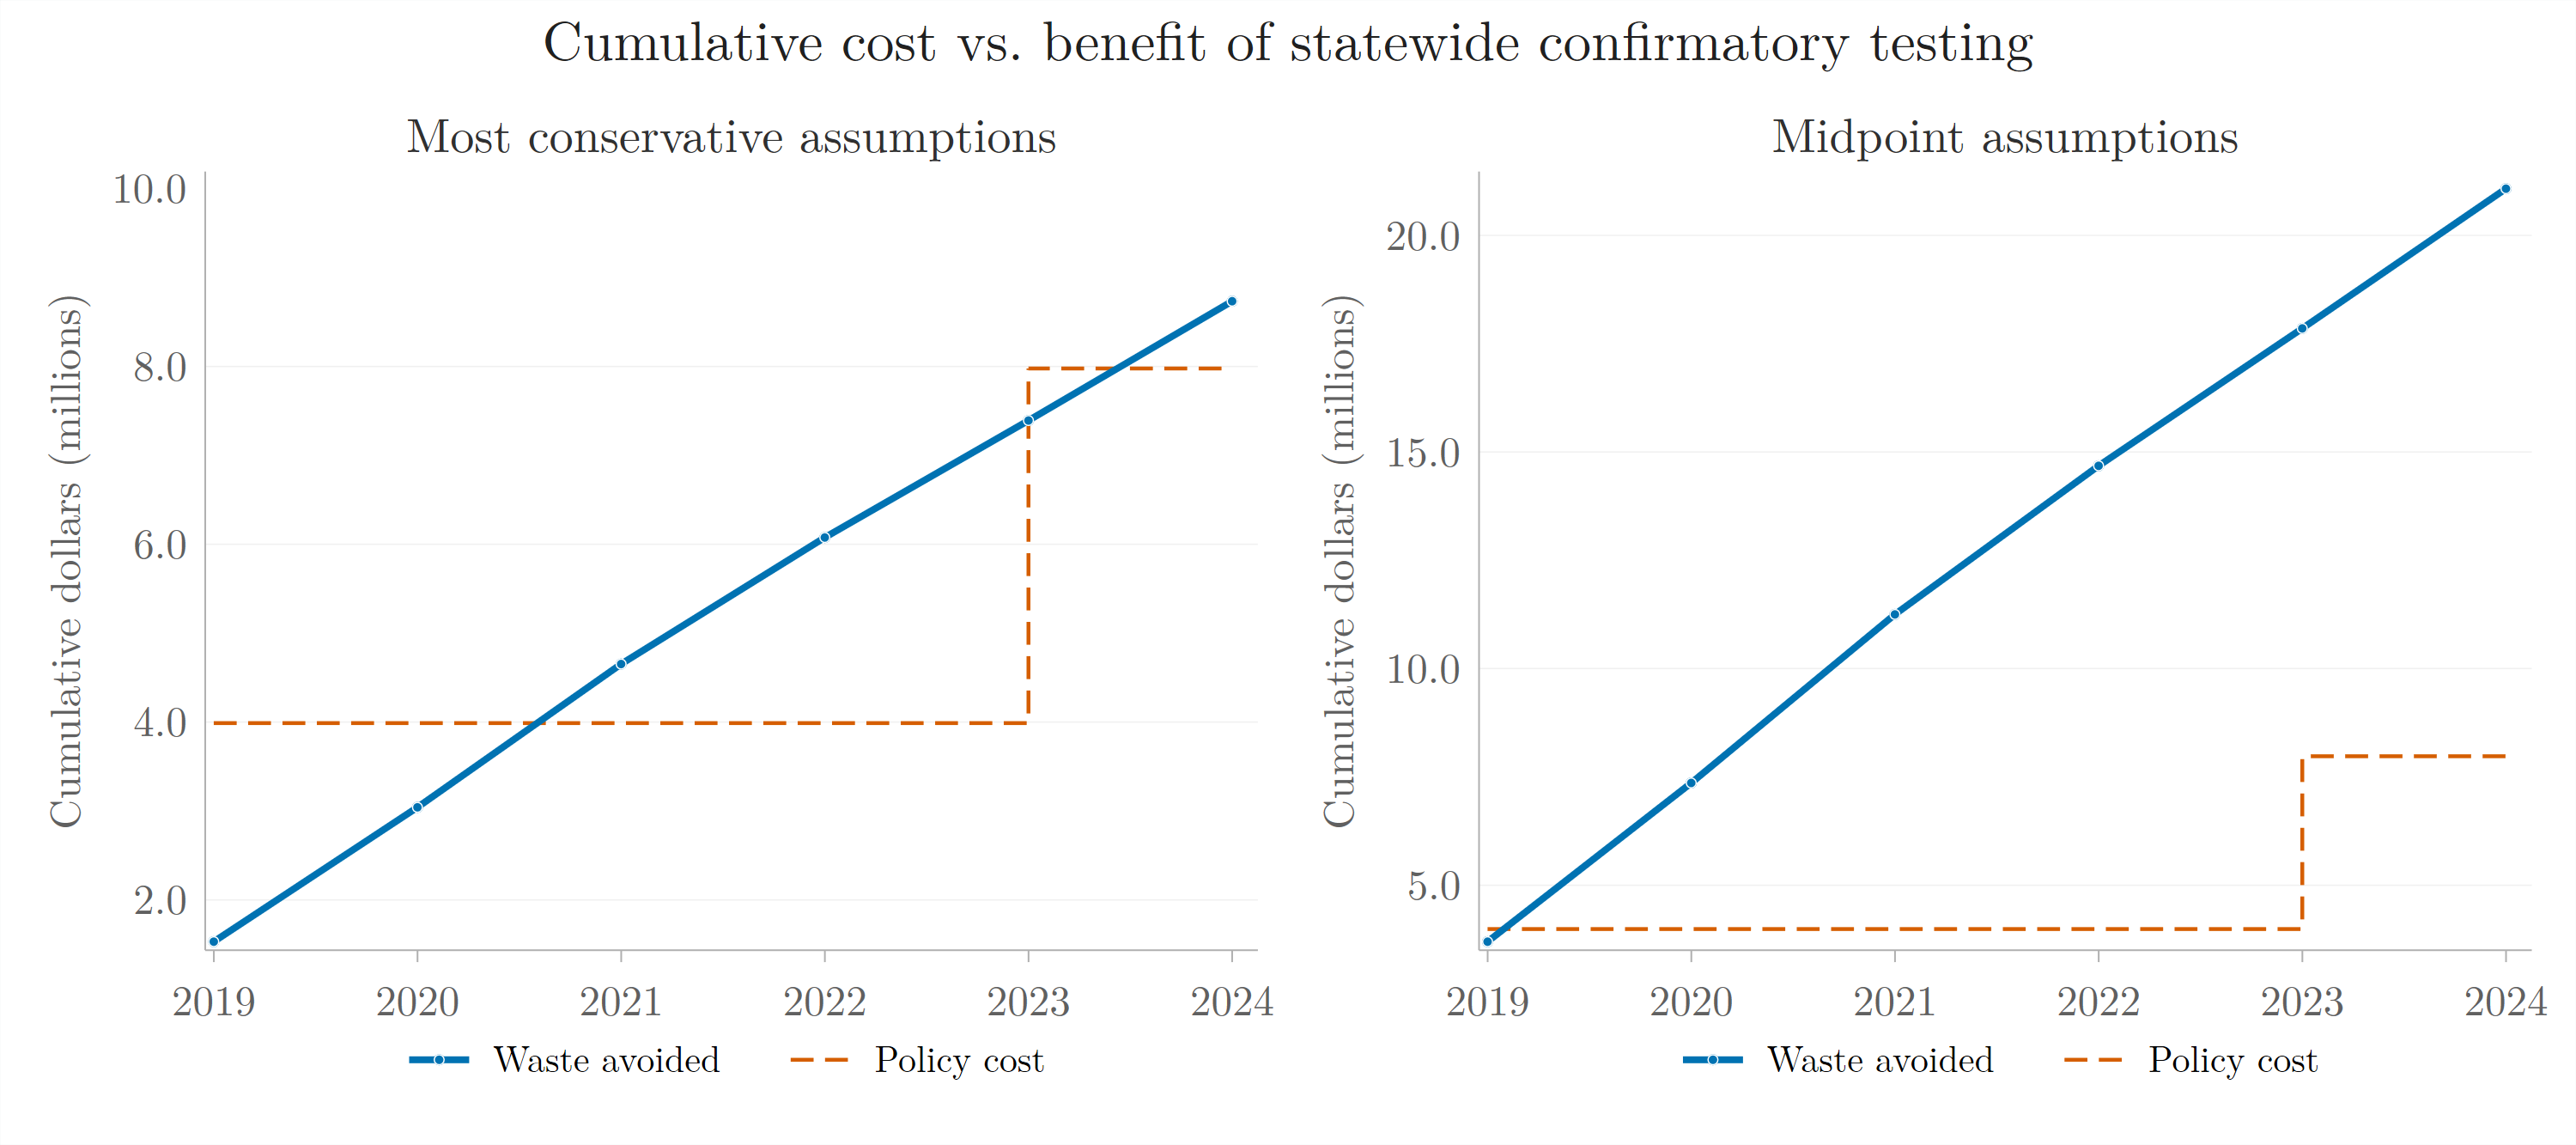
\includegraphics[width=\textwidth]{figures/costbenefit_timeseries.png}}{\textit{[run the Stata pipeline to generate this figure]}}
  \caption{Cumulative cost and benefit of statewide confirmatory testing from 2019: most conservative assumptions (left) and midpoint assumptions (right). The benefit line is cumulative colorimetric waste avoided; the cost line is the cumulative cost of the analyzers, purchased as a fleet up front and re-purchased every four years.}
  \label{fig:costbenefit}
\end{figure}

Figure~\ref{fig:costbenefit} models the effect of enacting this policy in 2019. The blue line represents cumulative waste avoided, while the red dashed line represents the cost of purchasing the requisite TruNarc analyzers for North Carolina police departments, and repurchasing the analyzers every 4 years. The left panel uses the most conservative assumptions; the right panel uses the midpoint of every assumption. In both, cumulative benefit overtakes cumulative cost and the gap widens over time. Even under our most conservative assumptions, and despite a steady decline in drug arrests over the sample period (from 38,101 in 2019 to 29,934 in 2024), our policy proposal breaks even within three years of enactment.


\section{Conclusion}
Under the most conservative possible set of assumptions and accounting for strictly economic costs to the state of North Carolina, a policy of eliminating colorimetric tests while maintaining the same level of drug testing in the state would save roughly \$500,000 annually. Even with a high upfront investment in drug scanners, the state would break even on its investment within three years. 

Our estimate of avoided costs would certainly be higher if we included private externalities (i.e. lost wages) as a result of arrests based on false positive drug tests, and our proposed policy alternative may not be the most cost effective policy---these factors could be explored in further expert analysis. Our report simply points out the millions of dollars of potential savings that would result from ceasing the use of colorimetric tests.

\end{document}
